%%%%%%%%%%%%%%%%%%%%%%%%%%%%%%%%%%%%%%%%%
% FRI Data Science_report LaTeX Template
% Version 1.0 (28/1/2020)
% 
% Jure Demšar (jure.demsar@fri.uni-lj.si)
%
% Based on MicromouseSymp article template by:
% Mathias Legrand (legrand.mathias@gmail.com) 
% With extensive modifications by:
% Antonio Valente (antonio.luis.valente@gmail.com)
%
% License:
% CC BY-NC-SA 3.0 (http://creativecommons.org/licenses/by-nc-sa/3.0/)
%
%%%%%%%%%%%%%%%%%%%%%%%%%%%%%%%%%%%%%%%%%


%----------------------------------------------------------------------------------------
%	PACKAGES AND OTHER DOCUMENT CONFIGURATIONS
%----------------------------------------------------------------------------------------
\documentclass[fleqn,moreauthors,10pt]{ds_report}
\usepackage[english]{babel}

\graphicspath{{fig/}}




%----------------------------------------------------------------------------------------
%	ARTICLE INFORMATION
%----------------------------------------------------------------------------------------

% Header
\JournalInfo{FRI Natural language processing course 2024}

% Interim or final report
\Archive{Project report} 
%\Archive{Final report} 

% Article title
\PaperTitle{LLM Prompt Strategies for Commonsense-Reasoning Tasks} 

% Authors (student competitors) and their info
\Authors{Žan Počkar, Amer Mujagić, and Ivan Nikolov}

% Advisors
\affiliation{\textit{Advisors: Aleš Žagar}}

% Keywords
\Keywords{Prompt Strategies, Prompt Evaluation}
\newcommand{\keywordname}{Keywords}


%----------------------------------------------------------------------------------------
%	ABSTRACT
%----------------------------------------------------------------------------------------

\Abstract{
With the rise in LLM usage, diverse optimization techniques have emerged. In order to evaluate and compare the efficiency of different prompt strategies, we first needed to describe what commonsense-reasoning tasks are. After describing the tasks we made a selection of different prompt strategies which required us reviewing the different strategies and choosing the ones that seemed to be both in popular use and different enough so that these evaluations could be extended to different sub-types of mentioned strategies. After choosing the strategies, we also choose models and datasets to test the strategies on, and reviewed possible evaluation methods.
}

%----------------------------------------------------------------------------------------

\begin{document}

% Makes all text pages the same height
\flushbottom 

% Print the title and abstract box
\maketitle 

% Removes page numbering from the first page
\thispagestyle{empty} 

%----------------------------------------------------------------------------------------
%	ARTICLE CONTENTS
%----------------------------------------------------------------------------------------

\section*{Introduction}
	Artificial language models especially large language models (LLMs) have in recent time vastly improved at tackling many tasks when provided with substantial training material. Yet enhancing their commonsense remains difficult. This paper explores approaches to nurture more natural reasoning in these models.

    Commonsense reasoning, the ability to understand and make judgments based on everyday knowledge and experiences, is a crucial aspect of human intelligence. While humans effortlessly apply this knowledge in their daily lives, imparting this ability to LLMs is a complex task. This paper investigates methods such as Chain of Thought (CoT), in-context learning, and plan-and-solve techniques to enhance model performance in tasks requiring common sense knowledge. To better analyse the results we will start our research with a Unicorn LLM\cite{Unicorn}. 

    In this paper we will firstly designing experiments to evaluate the effectiveness of each strategy. Later we will analyzing Unicorns’s reasoning processes, and document how different prompting techniques influence the outcomes. A key aspect of this work is the selection of an appropriate commonsense reasoning dataset. After considering several options, we choose the Rainbow \cite{Rainbow} benchmark, as this benchmark is a universal commonsense reasoning benchmark that brings together six existing commonsense reasoning tasks.


%------------------------------------------------
\section*{Problem}

Commonsense reasoning in Large Language Models (LLMs) is a complex problem due to the implicit and context-dependent nature of commonsense knowledge. For instance, consider the sentence “The ice cream was too hot to eat.” Humans intuitively understand this sentence is likely incorrect because ice cream is typically cold. However, an LLM might not flag this as an anomaly unless it has been explicitly trained on similar examples or has learned to associate certain objects with their typical properties.

Another challenge is the representation and utilization of commonsense knowledge in LLMs. LLMs learn from the patterns in the data they are trained on, so the size and quality of the training dataset significantly influence their performance. However, encoding commonsense knowledge into a machine-readable format that an LLM can learn from is not straightforward. For example, understanding that “people usually sleep at night” requires the model to learn not just the concepts of “people,” “sleep,” and “night,” but also the typical association between these concepts.

Lastly, the evaluation of commonsense reasoning in LLMs is a significant challenge. Traditional evaluation metrics may not adequately capture the nuances of commonsense reasoning. For instance, if an LLM generates the sentence “The man opened his umbrella because it was raining,” it demonstrates an understanding of the causal relationship between rain and using an umbrella. However, quantifying this understanding and comparing it across different models or tasks is not trivial, necessitating the development of more sophisticated evaluation metrics and benchmarks.

\section*{Prompting Techniques}

Prompts techniques are the proposed input structures that guide LLMs to produce outputs with the desired form and content quality. That is, to simplify, we can say that we use different prompting techniques to "program" LLM inputs by following specific patterns in order to obtain an output. \cite{prompttechniques}

\subsection*{Few-shot prompting}
Few-shot prompting \cite{Few-shot} is a prompting technique that consists of adding examples of how a response to a problem would look a number of times before stating the problem we want solved. Depending on the number of examples we give we can more specifically define our technique as n-shot learning, where n is the number of examples we gave before asking the question. Techniques similar in concept to few-shot prompting are zero-shot prompting (just asking the question directly) or one-shot prompting (adding a single example to a prompt). 
Examples that show the differences between zero-shot, one-shot and few-shot prompts can be seen in Figure 3.

\subsection*{Chain of thought}
Chain of Thought (CoT) \cite{CoT} prompting involves adding a series of intermediate reasoning steps to the intended task. It has been shown to improve performance in more complex prompts.
These intermediate reasoning steps can be thought of as giving an answer to a similar problem but with detailed steps on how to get to that answer as shown in Figure 1. This is similar to few-shot prompting, which also provides examples of answers to similar questions, however few-shot prompts include less detail that is they usually provide only questions and answers, no intermediate reasoning steps in between. \cite{CoT}

\begin{figure}[!h]\centering
	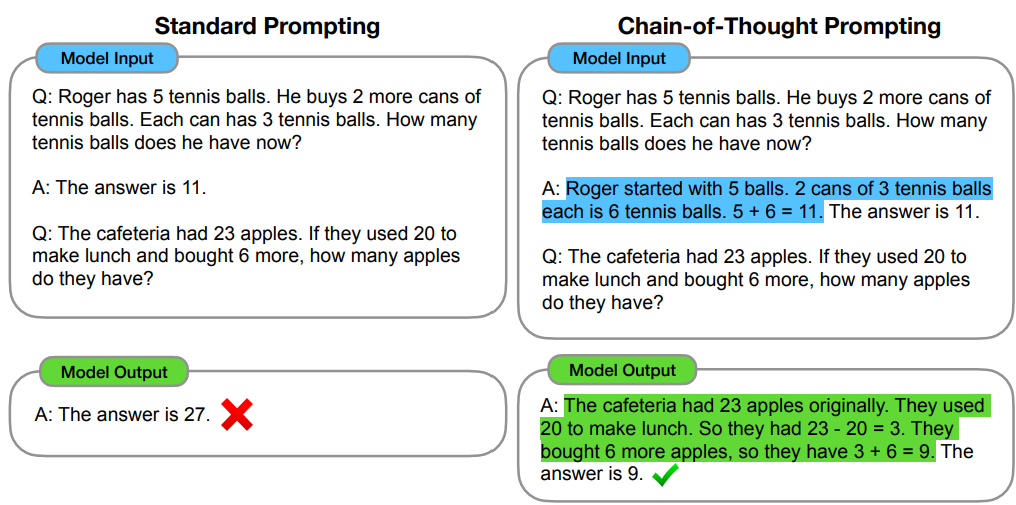
\includegraphics[width=\linewidth]{Example_CoT.png}
	\caption{Example of a Chain of Thought prompt versus a regular prompt}
	\label{fig:column}
\end{figure}

\subsection*{Plan and solve}
The plan and solve \cite{plansolve} prompting technique breaks up our prompt into multiple prompts. It starts with a prompt that constructs a plan to solve the stated problem, after which it uses the generated plan to guide the model into providing the final solution. An example of this approach is shown in Figure 2

\begin{figure}[!h]
    \centering
    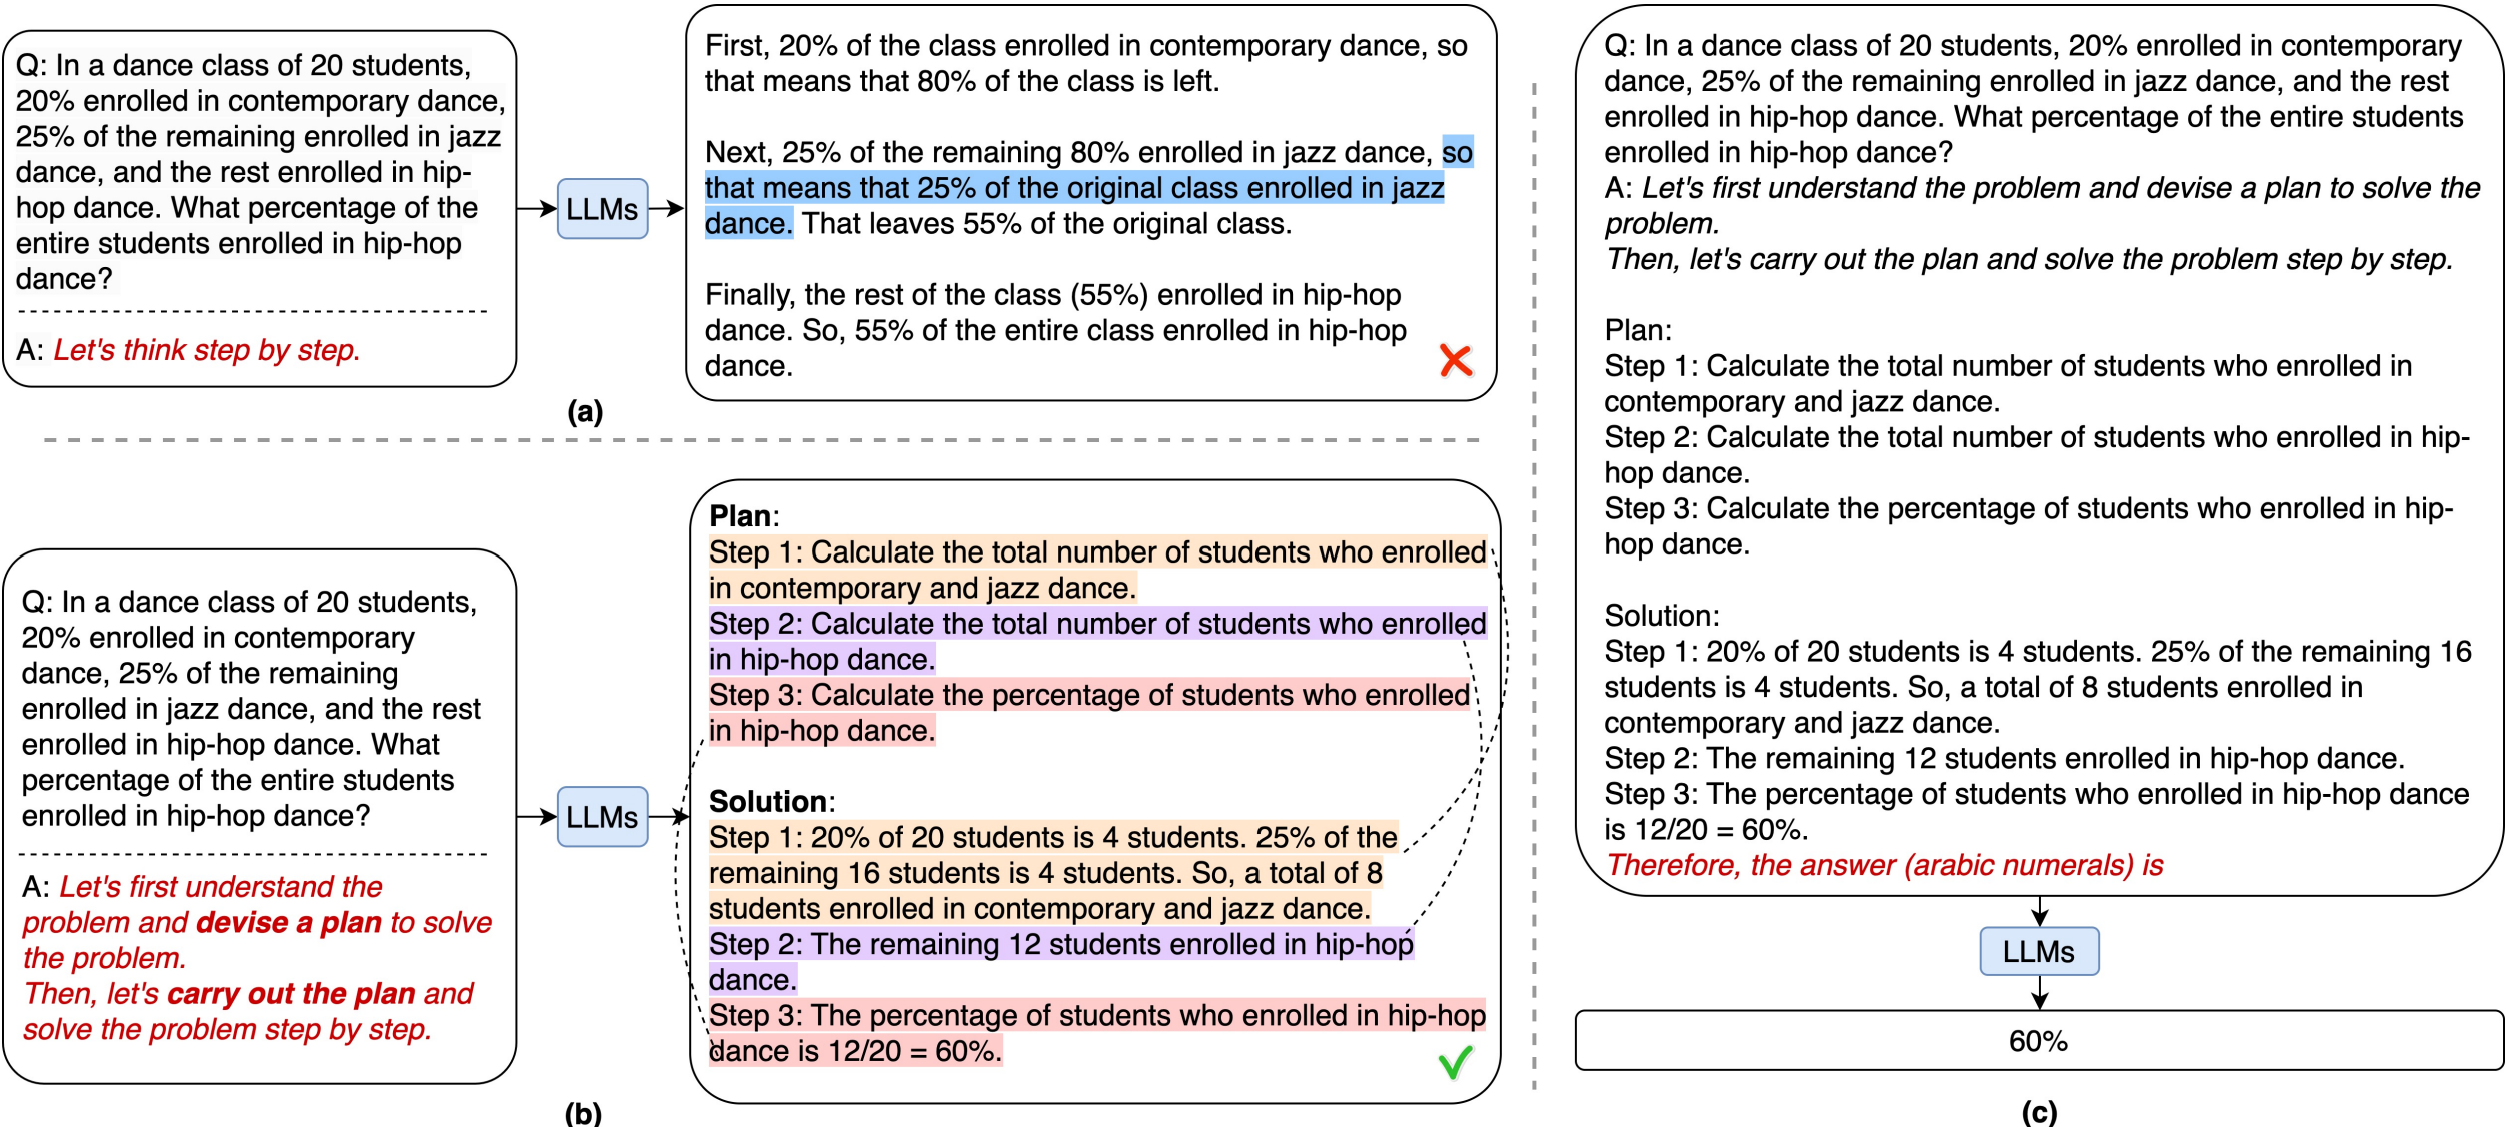
\includegraphics[width=\linewidth]{fig/image.png}
    \caption{Plan and solve prompt series example}
    \label{fig:colum}
\end{figure}

\subsection*{Three of thoughts}
Tree of Thoughts (ToT) \cite{ToT} is a technique that is based one exploring multiple reasoning paths over thoughts. ToT frames any problem as a search over a tree, where each node is a state representing a partial solution with respect to the input and the sequence of previous thoughts. A specific construction of ToT can be divided into solving four sub-problems:
\begin{enumerate}
    \item Decomposition of the intermediate process into thought steps
    \item Potential thought generation based on each individual state
    \item State evaluation
    \item Choice of search algorithm 
\end{enumerate}

The differences between similar strategies are shown in Figure 3.
\begin{figure}[!h]\centering
	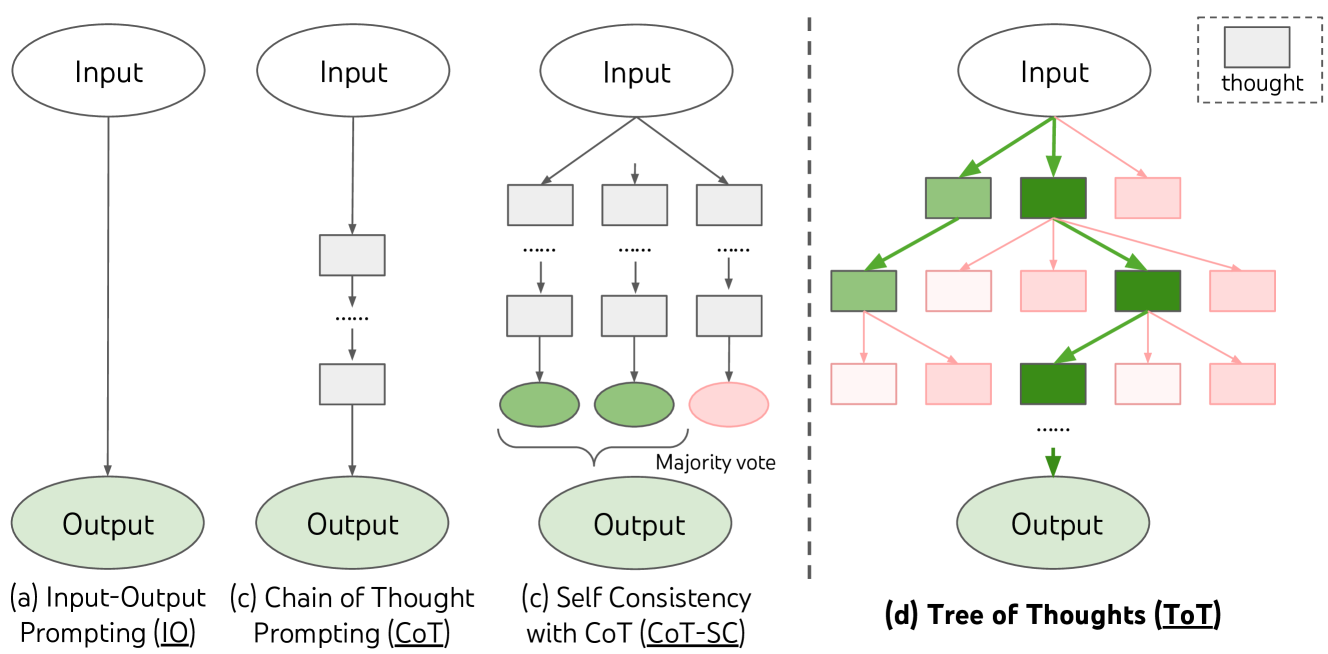
\includegraphics[width=\linewidth]{fig/x1.png}
	\caption{Differences between IO, CoT, CoT-SC and ToT}
	\label{fig:column}
\end{figure}

\subsection*{Directional Stimulus prompting}
This prompting technique adds a component named "directional stiumulus" to the prompt. The goal is to provide guidance for a specific prompt. This technique adds hints and clues to the input query to try and guide the model to producing a higher quality response. This method differs from other methods as it doesn't add additional knowledge to the prompt. \cite{directional} An example of this approach is shown in Figure 4.

\vspace{10pt}

\begin{figure}[!h]
    \centering
    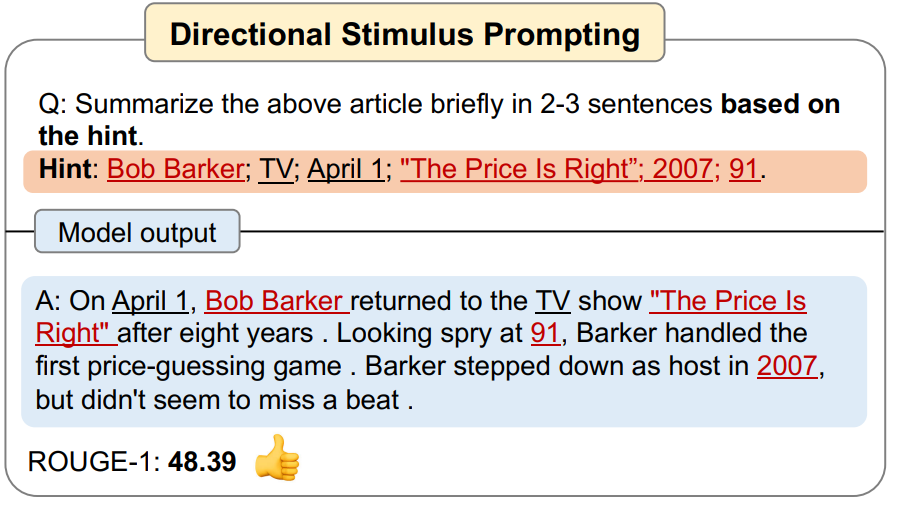
\includegraphics[width=\linewidth]{fig/directional.png}
    \caption{Example of directional stiumulus prompting}
    \label{fig:column}
\end{figure}


\begin{figure}[!h]\centering
	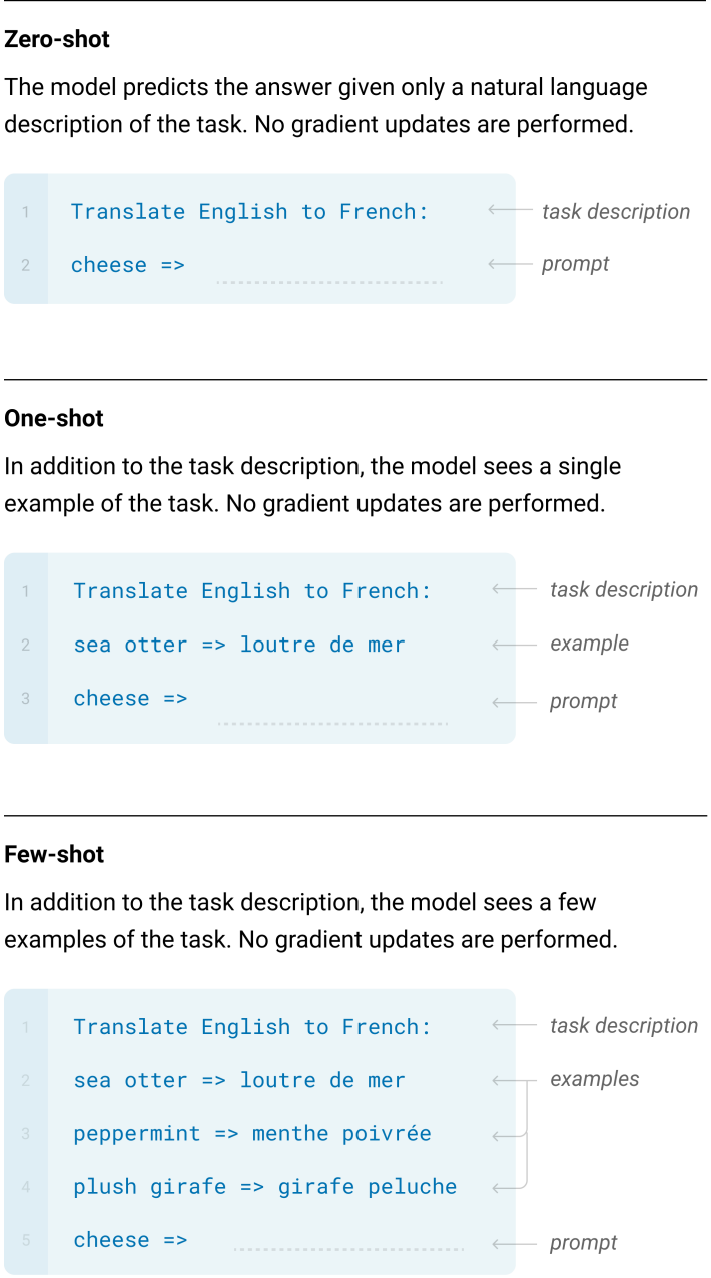
\includegraphics[width=\linewidth]{fig/few-shot-new.png}
	\caption{Examples of zero-shot, one-shot and few-shot prompts}
	\label{fig:column}
\end{figure}


\section*{Datasets}
Because commonsense reasoning is a complex topic and encompasses a wide collection of different tasks, it is difficult to generate a dataset that will evaluate the model's generalization abilities.

The Winograd schema challenge \cite{levesque2012winograd} was the standard for testing the commonsense reasoning, however from 2019 it is considered defeated since numerous transformer-based models achieved over 90\% accuracy. \cite{beaten_winograd}
For that reason, we will use more recent and challenging datasets.

On the one side, we have different SOTA methods \cite{CoT} evaluated on task specific datasets like GSM8K \cite{GSMK8}. This dataset focuses on linguistically diverse grade school math problems created by human problem writers.

On the other side, there are benchmarks that combine multiple commonsense datasets. For this project we will use Rainbow which is a suite of commonsense benchmarks that contain multiple choice question-answering datasets.
Rainbow contains the following datasets

\begin{itemize}
    \item $\alpha$NLI \cite{alphaNLI} - tests abductive reasoning in narratives. Models need to find the best explanation among the presented options connecting a beginning and ending;
    \item  CosmosQA \cite{Tian2020} — asks commonsense reading comprehensions about narratives in everyday situations
    \item HellaSWAG \cite{Zellers2020} — models need to find the most plausable ending to a short content.
    \item PIQA \cite{Bisk2020} — question answering benchmark for commonsense reasoning.
    \item SocialIQa \cite{socialIQA} — commonsense reasoning about social situations and interactions
    \item WinoGrande \cite{WinoGRANDE} — large-scale collection of Winograd schema-inspired problems that test reasoning about social and physical interactions.
\end{itemize}

Other possibilities for testing commonsense reasoning are the GLUE \cite{GLUE} and SuperGLUE \cite{supeglue} datasets, which are benchmarks for general language understanding systems.



%----------------------------------------------------------------------------------------
%	REFERENCE LIST
%----------------------------------------------------------------------------------------
\bibliographystyle{unsrt}
\bibliography{report}


\end{document}